% questions.tex —— 1977 年·新疆卷（文科） · 题目内容片段（无答案）
% 由 tools/generate_projects.py 依来源总账自 1977/1977_数学真题_新疆文_试题.md 生成，勿手改（改源 MD 后重跑）


\gkpart{新疆维吾尔自治区（文科）}

\begin{gktip}
\textbf{来源说明}：本题面依据固定源 PDF《1977新疆文.pdf》第 1—5 页逐题转录。源卷为解答汇编书籍的书页扫描（书页码 106—109，第 5 页未见页码），性质是题面与解答连续出现：每题题面后紧随完整源解答；本文件只转录题面，解答经独立复算写入配套答案要点与解析正文。原卷标题仅印“新疆维吾尔自治区（文科）”，未印总标题与年份，括注“文科”即科类范围。原卷题号用汉字“一”至“七”，本库转录为阿拉伯数字 1—7；各题分值按原卷照录，全卷合计 100 分；原卷无附加题、参考题。
\end{gktip}

\par\medskip

\begin{question}
\gkti{1}\textbf{（15 分）} 解方程：

\nopagebreak[4]
\[
\frac{x-1}{x+1}-\frac{5}{1-x}=\frac{4}{x^2-1}
\]

\end{question}
\begin{question}
\gkti{2}\textbf{（16 分）} 红心大队贫下中农坚决顶住“四人帮”对农业学大寨运动的干扰和破坏，积极发展养猪事业，1974 年底全大队养猪 200 头，到 1976 年底发展到 1200 头，求平均每年的增长率，（精确到 $1\%$）

\end{question}
\begin{question}
\gkti{3}计算：

\Needspace{5\baselineskip}
（1） 化简：（7 分）

\nopagebreak[4]
\[
\frac{\frac{3}{4}(ab)^{-\frac{1}{3}}\left(\frac{4}{9}a^4b^{\frac{2}{3}}\right)^{\frac{1}{2}}}{2a^3\sqrt{a^2}}
\]

\begin{gktip}
\textbf{源注}：原卷括号内该因式印作“$a^4d^{\frac{2}{3}}$”，源解答按 $a^4b^{\frac{2}{3}}$ 展开计算——字母 $b$ 与前一因式 $(ab)^{-\frac{1}{3}}$ 一致，且恰使化简结果中 $b$ 的指数归零，系 $b$、$d$ 形近排印之误，本卷按 $b$ 转录。
\end{gktip}

（2） 已知 $\lg 2=0.3010$，求 $\lg\sqrt{800}$（7 分）

\Needspace{0.4\textheight}
\end{question}
\begin{question}
\gkti{4}\textbf{（16 分）} 求证：四边形对边中点的连线互相平分。

\begin{gktip}
原源 PDF 第 3 页附有四边形及对边中点连线示意图；LaTeX 版按源图重绘。
\end{gktip}
\nopagebreak[4]
\begin{center}% 1977 年新疆卷（文科）第四题：四边形 ABCD，E、F、M、N 分别为 AD、AB、BC、CD 的中点，
% 实线 EM 与 FN，虚线 EF、FM、MN、NE 及对角线 BD（按源卷第 3 页布局：A 左上、D 右上、B 左下、C 右下）
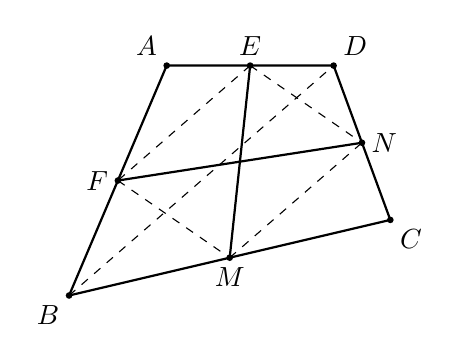
\begin{tikzpicture}[scale=1.0]
  \coordinate (B) at (0,0);
  \coordinate (A) at (1.24,2.92);
  \coordinate (D) at (3.36,2.92);
  \coordinate (C) at (4.08,0.96);
  \coordinate (E) at (2.30,2.92);
  \coordinate (F) at (0.62,1.46);
  \coordinate (M) at (2.04,0.48);
  \coordinate (N) at (3.72,1.94);
  \draw[thick] (A)--(D)--(C)--(B)--cycle;
  \draw[thick] (E)--(M);
  \draw[thick] (F)--(N);
  \draw[dashed] (E)--(F);
  \draw[dashed] (E)--(N);
  \draw[dashed] (F)--(M);
  \draw[dashed] (M)--(N);
  \draw[dashed] (B)--(D);
  \fill (A) circle (1.2pt) node[above left] {$A$};
  \fill (D) circle (1.2pt) node[above right] {$D$};
  \fill (C) circle (1.2pt) node[below right] {$C$};
  \fill (B) circle (1.2pt) node[below left] {$B$};
  \fill (E) circle (1.2pt) node[above] {$E$};
  \fill (F) circle (1.2pt) node[left] {$F$};
  \fill (M) circle (1.2pt) node[below] {$M$};
  \fill (N) circle (1.2pt) node[right] {$N$};
\end{tikzpicture}
\end{center}
\nopagebreak[4]
\end{question}
\begin{question}
\gkti{5}\textbf{（10 分）} 解方程组

\nopagebreak[4]
\[
\begin{cases}
2x-3y=9\\
3x+4y=5
\end{cases}
\]

\Needspace{0.4\textheight}
\end{question}
\begin{question}
\gkti{6}\textbf{（14 分）} 红升人民公社小水库拦水坝的横断面为梯形，坝顶宽 2.5 米，坝高 4 米，迎水坡、背水坡与水平面的夹角分别是 $30^\circ$ 和 $45^\circ$，求坝底的宽。（精确到 $0.1$ 米）

\begin{gktip}
原源 PDF 第 4 页附有拦水坝横断面示意图，坝顶标有 2.5 的尺寸标注，左侧绘有水面示意短线；LaTeX 版按源图重绘。
\end{gktip}
\nopagebreak[4]
\begin{center}% 1977 年新疆卷（文科）第六题：拦水坝梯形横断面 ABCD（AD 为坝顶，BC 为坝底），
% AE、DF 为坝高的垂线（虚线），左侧水面示意短线，角 B=30°、角 C=45°，
% 坝顶上方标 2.5 尺寸线（按源卷第 4 页布局；比例约 1:2.2，非严格尺寸）
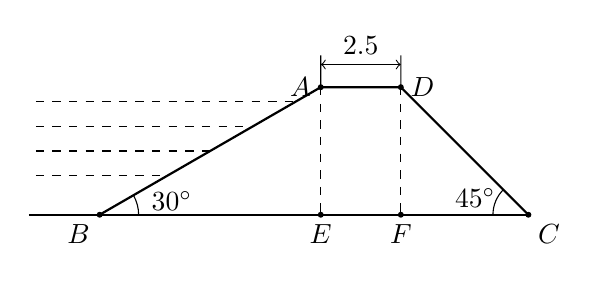
\begin{tikzpicture}[scale=0.9]
  \coordinate (B) at (0,0);
  \coordinate (E) at (3.12,0);
  \coordinate (F) at (4.25,0);
  \coordinate (C) at (6.05,0);
  \coordinate (A) at (3.12,1.8);
  \coordinate (D) at (4.25,1.8);
  \draw[thick] (-1.0,0)--(C);
  \draw[thick] (B)--(A)--(D)--(C);
  \draw[dashed] (A)--(E);
  \draw[dashed] (D)--(F);
  % 水面示意短线（迎水坡一侧）
  \draw[dashed] (-0.9,0.55)--(0.95,0.55);
  \draw[dashed] (-0.9,0.90)--(1.56,0.90);
  \draw[dashed] (-0.9,1.25)--(2.17,1.25);
  \draw[dashed] (-0.9,1.60)--(2.77,1.60);
  % 坝顶 2.5 尺寸标注
  \draw[thin] (A)--(3.12,2.25);
  \draw[thin] (D)--(4.25,2.25);
  \draw[<->] (3.12,2.12)--(4.25,2.12) node[midway,above] {$2.5$};
  % 角标注
  \draw (0.55,0) arc[start angle=0,end angle=30,radius=0.55];
  \node at (1.02,0.20) {$30^\circ$};
  \draw ([shift={(180:0.5)}]C) arc[start angle=180,end angle=135,radius=0.5];
  \node at (5.30,0.24) {$45^\circ$};
  \fill (A) circle (1.2pt) node[left] {$A$};
  \fill (D) circle (1.2pt) node[right] {$D$};
  \fill (B) circle (1.2pt) node[below left] {$B$};
  \fill (E) circle (1.2pt) node[below] {$E$};
  \fill (F) circle (1.2pt) node[below] {$F$};
  \fill (C) circle (1.2pt) node[below right] {$C$};
\end{tikzpicture}
\end{center}
\nopagebreak[4]
\Needspace{0.4\textheight}
\end{question}
\begin{question}
\gkti{7}\textbf{（15 分）} 已知，直线过 $A(2,-5)$ 和 $B(-3,0)$ 两点，求此直线方程，并指出直线的斜率 $K$=？，直线与 $OX$ 轴正方向的夹角 $\alpha$=？

\begin{gktip}
原源 PDF 第 5 页解答旁附有坐标系与直线示意图；LaTeX 版按源图重绘并移至题面处。
\end{gktip}
\nopagebreak[4]
\begin{center}% 1977 年新疆卷（文科）第七题：直线 y=-x-3 过 B(-3,0) 与 A(2,-5) 的坐标系示意图，
% 两轴带箭头，坐标轴上绘单位刻度点（按源卷第 5 页布局）
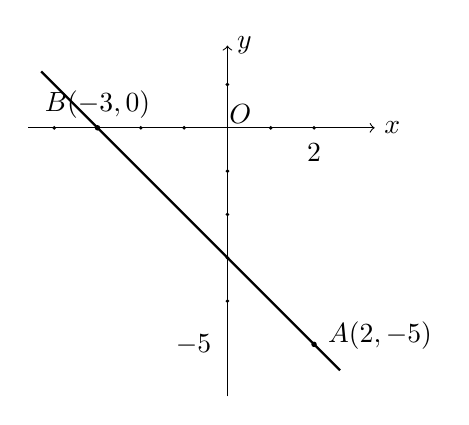
\begin{tikzpicture}[scale=0.55]
  \draw[->] (-4.6,0)--(3.4,0) node[right] {$x$};
  \draw[->] (0,-6.2)--(0,1.9) node[right] {$y$};
  \node at (0.30,0.32) {$O$};
  % 单位刻度点
  \foreach \xx in {-4,-2,-1,1,2} \fill (\xx,0) circle (1.3pt);
  \foreach \yy in {1,-1,-2,-3,-4} \fill (0,\yy) circle (1.3pt);
  \node[below] at (2,-0.15) {$2$};
  \node[left] at (-0.15,-5) {$-5$};
  % 直线 y=-x-3
  \draw[thick] (-4.3,1.3)--(2.6,-5.6);
  \fill (-3,0) circle (1.8pt) node[above] {$B(-3,0)$};
  \fill (2,-5) circle (1.8pt);
  \node[right] at (2.1,-4.8) {$A(2,-5)$};
\end{tikzpicture}
\end{center}
\nopagebreak[4]

\end{question}